\chapter{Research Goal, Aim and Objectives}
Based on the environmental challenge, (minimize the environmental impacts) the state of the art and the identified knowledge gap, the \textbf{goal of this thesis will be to understand the the role regional spatial planning can play in facilitating circular economy practices}. %re-write this. pay attention to facilitating
By describing and analyzing how secondary resources (waste) flow in a city-region it will be possible to explore how the location of different socio-economic activities contribute to closing material loops. \par
By exploring the relevance of the spatial patterns, this project will contribute to understand how planning instruments could be integrated with material flow analysis.\par


\begin{figure}[h!]
    \centering
    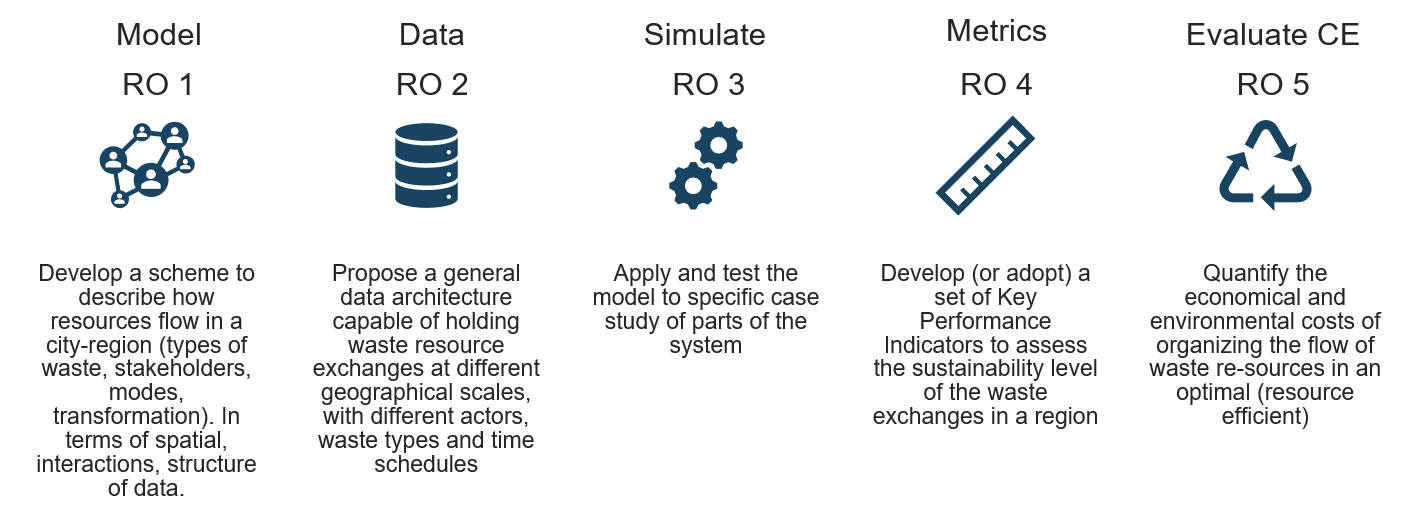
\includegraphics[width=0.8\textwidth]{sections/asset/ros.PNG}
    \caption{Short description of research objectives}
    \label{fig:research objectives}
\end{figure}

Most of the socio-economic process that currently exist, are still part of the so-called linear economy model, where a raw material is produced, then sold and later disposed as waste; a by-product of production or consummation that in most of times does not have any economical value for society. As explained before the paradigm of Circular Economy implies that there are different strategies to be implemented make this process to close the loop of resources between production and consummation. The ecosystem of strategies to be adopted under this new paradigm is vast and need to be applied in the 3 stages of a life of any product: at the stage of development, using local and waste resources, maximizing the life span of a product and ensuring that after the product is no longer used, its components could be easily dismantled and reused again. \par
In this project, the contribution to the Circular Economy paradigm will be focused on trying to close by exploring the role of urban and regional planning. \par
From economic geography theory it has been acknowledged that the location of some economic activities follow certain rationale. Some industries tend to experience different benefits by co-locating one next to the other. Industrial and Eco-industrial parks has shown, that they can be used as tools to increase production efficiency. Water, electricity and other resources are shared or used in a smarter why which result in symbiotic relationships. \par
Since not all socio-economic activities are co-located, but sparse in space, resources and waste resources flow in space creating a demand for transporting these materials. \par
Thanks to the advancements in computing and digital technologies, now more than ever it has become easier to know what and how much is being produced, what and how much waste is being produced and also, we might be at the stage of knowing where these events occur. The possibility of having this information, creates an enormous potential to study the role of space to reduce waste creation. By having the possibility of mapping, analyzing and simulations different scenarios, practitioners and policy makers can be offered analytical tools to work towards more sustainable futures. \par

\section{Research objectives}

In order to  successfully reach the goal of this research, the project the following objectives:
\begin{enumerate}

    \item 
    Develop an information scheme to describe how resources flow in a city-region. The scheme should be able to hold information about different waste types, stakeholders, waste uses, how is transported and other attributes. The scheme developed should hold geographical information and how the different actors and components in the system relate to each other.
    
    \item 
    Propose a general data architecture capable of holding waste resource exchanges at different geographical scales, with different actors, waste types and time schedules. 
    
    \item 
    Apply and test the spatial model  %(datamodel)
    to an specific case study. The case study will contribute to test to what extent the data model is capable of holding information of a part of a system. The case study must be geographically constrained, but also in terms of the waste typology. 
    %--> TASK: Identify, collect, organize data to be used to describe how resources flow in a city-region --> TASK: Quantify, describe, map the waste resources flowing in a city-region. TASK2: Model and simulate how waste resources should flow to attain high levels of sustainability by maximizing the use of waste flows. 
    
    \item 
    Develop (or adopt) a set of Key Performance Indicators to assess the sustainability level of the waste exchanges in a region. These metrics should be able to capture the performance of a region or urban area in terms of usage of waste materials. 
    
    \item Quantify economical and environmental costs of organizing the flow of waste resources under different scenarios. By understanding and comparing how different scenarios perform different, the learning could be used to plan better city-regions.

\end{enumerate}


